% $Id: PhysGrid_background.tex,v 1.5 2002/05/23 20:07:18 jwolfe Exp $

\section{Background}


  Earth system models use a variety of different discrete grids to represent
continuous physical space. The ESMF physical grid is 
responsible for maintaining information about physical coordinate based 
discretizations of simulation domains. Components may include and use 
additional grid information internally, however, the only physical grid 
information that framework operates on will come through physical grid elements. 

  The information that the framework needs to represent in physical grids is quite
extensive. Coupled components need to be able to provide physical grid information
that is sufficiently detailed for regridding operators (see Regrid) which
transfer field data between the components.  The primary ESMF codes employ
finite-difference and finite-volume grids, spectral grids, unstructured
land-surface grids and ungridded observational networks.  This requires the
physical grid to support an extensive range of metric terms (e.g. grid spacings,
areas and volumes) and grid masks.

 The grids used in Earth system models evolve continually. The physical grid
of ESMF will be extensible, so that support for future
grids can be added to the framework over time.

\subsection{Location}

  The physical grid is a part of the "Fields and Grids" portion of the ESMF
infrastructure layer. The physical grid interacts closely with the index spaces in the 
distributed grid facility; the creation of a distributed grid precedes the 
creation of a physical grid.  Most Fields exist at locations described via physical grids.  
Regrid typically uses physical grid information. The ESMF Control
superstructure element supports the passing of physical grid information between
components. Field values with different physical grid settings and belonging
to different components can be exchanged through the Coupler element of the 
superstructure.

\subsection{Scope}

Physical grids do not cover domain decomposition or specification of grid
topology; these are covered by distributed grids. Also, although most fields
in ESMF have a natural physical grid associated with them, there are
some cases where a physical grid is not relevant. For example
a hypothetical assimilation system optimization scheme could be adapted
into an ESMF component. Many optimization schemes work in a linear-algebra
space that is far removed from the underlying physical space, so fields
that are operated on by this component might not have a realizable
physical grid.

\subsection{Examples}


\begin{figure}
\includegraphics[trim= 100 200 100 -100,width= 5.5in]{hgridmontage.eps}
\caption{
Sketches representing various key horizontal, physical grids that ESMF will
need to support. The set includes grids that are represented
in functional form (for example Spherical Harmonics based
grids), grids that are regular but that are typically 
represented as numerical values (for example the four
curvilinear orthognal grids in the right panel) and grids for
which no underlying functional form exists. These latter
grids are illustrated in the two lower panels in the left column.
One panel (middle left) depicts a land surface grid, its
grid layout typically reflects catchment basin topography,
the other panel (lower left) illustrates a independent
set of grid locations that is associated with a set of 
floats drifting in the ocean. The family of grids illustrated
encompasses many other common grids that are not shown, for example
cartesian and cylindrical grids.
\label{fig:pg_reqdoc:hgridmontage}
}
\end{figure}

Gridding is a fumdamental aspect of models supported by ESMF.
Figure \ref{fig:pg_reqdoc:hgridmontage} shows a number of example 
horizontal grids that must be supported by ESMF. 
Figure \ref{fig:pg_reqdoc:vgridmontage} illustrates a subset of the 
vertical gridding schemes that will be supported by ESMF.
For components to interoperate they will need to be able to exchange detailed 
information representing specific configurations of the grid types
shown in the figure.
 
 For example, under ESMF an atmospheric component employing a spectral
algorithm with spherical harmonic basis functions could be coupled
together with a land surface component using a catchment area based grid
and with an ocean circulation component using a rotated pole grid.
As discussed in the ESMF Regrid requirements chapter \ref{}, exchanging information 
between these components, under appropriate conservation side-conditions, requires 
detailed information about the grid discretization. For this example the
information that is required includes such items as
\begin{description}
\item the areas of each of the cells of the land grid and
their spatial extent, 

\item the truncation level of the spherical harmonic
series in the atmospheric model and the functional form of
used to define the spherical harmonic basis functions

\item the land and sea grid cell locations and areas in the ocean model
associated with both terms in the momentum equations and
thermodynamic terms.
\end{description}

Figure \ref{fig:pg_reqdoc:hgridmontage} also shows so-called ``ungridded''
information. Examples of ``ungridded'' data in ESMF derive from
ingestion of observations into components.
Ingesting and comparing to observational measurements entails
working with grids that are associated with point wise 
and track measurements, for example
\begin{description}
\item an assimilation system might need to
sample flow simulated in an atmospheric component in 
a manner consistent with radiosonde balloon netowrk measurements
or with satellite track data
\item an ocean state estimation system might need to sample and analyze
fields in a manner consistent with ship and satellite
track or current meter observations.
\end{description}
In these examples both horizontal and vertical physical grid remappings
may be required, in order to represent simulated data in the observational
space and vice-versa.

